\documentclass[12pt]{article}
\usepackage[utf8]{inputenc}
\usepackage[english]{babel}
\usepackage[export]{adjustbox}
\usepackage{amsmath}
\usepackage{amssymb}
\usepackage{anysize}
\marginsize{2cm}{2cm}{2cm}{2cm}
\usepackage{appendix}
\usepackage{cancel}
\usepackage{caption}
\captionsetup{labelfont={bf}}
\usepackage{cite}
\usepackage{color}
\usepackage{fancyhdr}
\pagestyle{fancy}
\fancyhf{}
\fancyhead[L]{
\includegraphics[scale = 0.3]{Images/NovaFctHor.png}}
\fancyhead[R]{\footnotesize Computer Vision}
\fancyfoot[L]{\footnotesize MEEC}
\fancyfoot[R]{\thepage}
\renewcommand{\footrulewidth}{0.4pt}
\usepackage{float}
\usepackage{graphicx}
\usepackage[colorlinks = true, plainpages = true, linkcolor = novablue, urlcolor = novablue, citecolor = novablue, anchorcolor = novablue]{hyperref}
\usepackage{indentfirst}
\usepackage[super]{nth}
\usepackage{siunitx}
\usepackage{subcaption}
\usepackage{titlesec}
\titleformat{\section}{\Large\bfseries}{\thesection}{1em}{}
\titleformat{\subsection}{\large\bfseries}{\thesubsection}{1em}{}
\titleformat{\subsubsection}{\normalsize\bfseries}{\thesubsubsection}{1em}{}

\usepackage[breakable]{tcolorbox}
\usepackage{listings}
\lstset{ 
    backgroundcolor=\color{cellbackground},
    basicstyle=\ttfamily\small,
    breakatwhitespace=false,
    breaklines=true,
    captionpos=b,
    commentstyle=\color{gray},
    escapeinside={\%*}{*)},
    keywordstyle=\color{blue},
    stringstyle=\color{dkgreen},
    frame=single,
    rulecolor=\color{cellborder},
}

\usepackage[utf8]{inputenc}

% Default fixed font does not support bold face
\DeclareFixedFont{\ttb}{T1}{txtt}{bx}{n}{12} % for bold
\DeclareFixedFont{\ttm}{T1}{txtt}{m}{n}{12}  % for normal

% Custom colors
\usepackage{color}
\definecolor{deepblue}{rgb}{0,0,0.5}
\definecolor{deepred}{rgb}{0.6,0,0}
\definecolor{deepgreen}{rgb}{0,0.5,0}

% Python style for highlighting
\lstset{
language=Python,
basicstyle=\ttm,
morekeywords={self},              % Add keywords here
keywordstyle=\ttb\color{deepblue},
emph={MyClass,__init__},          % Custom highlighting
emphstyle=\ttb\color{deepred},    % Custom highlighting style
stringstyle=\color{deepgreen},
frame=tb,                         % Any extra options here
showstringspaces=false
}

\definecolor{mGreen}{rgb}{0,0.6,0}
\definecolor{mGray}{rgb}{0.5,0.5,0.5}
\definecolor{mPurple}{rgb}{0.58,0,0.82}
\definecolor{backgroundColour}{rgb}{0.95,0.95,0.92}

% C style for highlighting
\lstdefinestyle{CStyle}{
    backgroundcolor=\color{backgroundColour},   
    commentstyle=\color{mGreen},
    keywordstyle=\ttb\color{deepblue},
    numberstyle=\tiny\color{mGray},
    stringstyle=\color{deepgreen},
    basicstyle=\footnotesize,
    breakatwhitespace=false,         
    breaklines=true,                 
    captionpos=b,                    
    keepspaces=true,                 
    numbers=left,                    
    numbersep=5pt,                  
    showspaces=false,                
    showstringspaces=false,
    showtabs=false,                  
    tabsize=2,
    language=C
}

\usepackage{tikz}
\usetikzlibrary{shapes.geometric, arrows, positioning}
\definecolor{lightblue}{RGB}{173, 216, 230}
\tikzstyle{block} = [draw, rectangle, minimum height=2.5em, minimum width=3.5em]
\tikzstyle{arrow} = [thick,->,>=stealth]
\tikzstyle{startstop} = [rectangle, rounded corners, minimum width=3cm, minimum height=1cm, text centered, draw=black, fill=blue!30]
\tikzstyle{process} = [rectangle, minimum width=3cm, minimum height=1cm, text centered, draw=black, fill=cyan!30]
\tikzstyle{decision} = [diamond, minimum width=3cm, minimum height=1cm, text centered, draw=black, fill=lightblue]

\definecolor{incolor}{HTML}{303F9F}
\definecolor{outcolor}{HTML}{D84315}
\definecolor{cellborder}{HTML}{CFCFCF}
\definecolor{cellbackground}{HTML}{F7F7F7}
\definecolor{novablue}{RGB}{0, 101, 189}
\definecolor{dkgreen}{RGB}{52,129,65}

\usepackage{lipsum}
\usepackage{tabularx}
\usepackage{booktabs}
\usepackage{makecell}
\usepackage{cleveref}

\newcommand{\sen}{\operatorname{\sen}}
\newcommand{\HRule}{\rule{\linewidth}{0.5mm}}
\renewcommand{\appendixpagename}{\LARGE Appendices}

\begin{document}
\bibliographystyle{IEEEtran}

% Cover Page
\begin{center}
    \begin{figure}
        \vspace{-1.0cm}
        
\includegraphics[scale = 0.055, left]{Images/NovaFctVer.png}
    \end{figure}
    \mbox{}\\[2.0cm]
    \textsc{\Huge Mestrado em Engenharia Eletrotécnica e de Computadores}\\[2.5cm]
    \textsc{\LARGE Computer Vision}\\[2.0cm]
    \HRule\\[0.4cm]
    {\large \bf {A Motion-Based Interactive Game Using Computer Vision and GPU Acceleration}}\\[0.2cm]
    \HRule\\[1.5cm]
\end{center}

\begin{flushleft}
    \textbf{Authors:}
\end{flushleft}

\begin{center}
    \begin{minipage}{0.5\textwidth}
        \begin{flushleft}
            Filipe Cavalheiro (70119)\\
            Diogo Novais (70118)
        \end{flushleft}
    \end{minipage}%
    \begin{minipage}{0.5\textwidth}
        \begin{flushright}
            \href{mailto:fs.cavalheiro@campus.fct.unl.pt}{\texttt{fs.cavalheiro@campus.fct.unl.pt}}\\
            \href{mailto:dm.novais@campus.fct.unl.pt}{\texttt{dm.novais@campus.fct.unl.pt}}
        \end{flushright}
    \end{minipage}
\end{center}

\vspace{5cm}

\begin{center}
    \large \bf 2025/2026 -- \nth{1} Semester, DEEC
\end{center}

\thispagestyle{empty}
\setcounter{page}{0}
\newpage

\tableofcontents
\newpage

\listoffigures
\newpage

\section{Introduction}

This project implements an interactive motion-based game that leverages
advanced computer vision techniques to create an engaging user experience. The
system combines face detection, pose estimation, template matching, and
GPU-accelerated image processing to enable players to control game elements
using body movements captured through a standard webcam.

The project demonstrates the practical application of multiple computer vision
algorithms, including deep neural networks (DNN) for detection tasks and custom
OpenCL kernels for high-performance image processing operations. The game
implements a "Simon Says" style interaction where players must position their
hands over colored squares based on text prompts, creating a challenging
exercise in both visual perception and physical coordination.

A video demonstatios of the project can be seen at:
\href{https://youtu.be/y8x0-IAdg58}{TAPDI - Apresentação do projeto}

\subsection{Project Objectives}

For this project we were tasked with using real time template matching using
the GPU and kernels in order to track and stabelize/center the games user in
the center of the screen at all times, at the same time pose estimation was
done via the OpenPose library having a ROI for analysis based on the location
of the users face, detected via a DNN. Finally a game of our choice, in this
case "Simon Says", must be implement with this technology in mind.

\section{Technical Architecture}

\subsection{System Overview} \label{subsec:System Overview}

The system architecture consists of several interconnected modules, each
responsible for specific computer vision tasks.
Figure~\ref{fig:system_architecture} illustrates the overall data flow through
the system.

\begin{figure}[H]
    \centering
    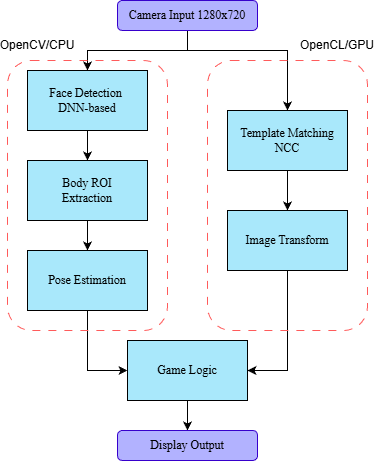
\includegraphics[width=0.6\textwidth]{./Images/System_Architecture.png}
    \caption{System architecture and data flow diagram}
    \label{fig:system_architecture}
\end{figure}

\subsection{Module Descriptions}

The multiple modules shown in \cref{fig:system_architecture} have are below
described:\\

\begin{itemize}
    \item Face Detection DNN-based (\cref{subsec:DNN-Based Detection Pipeline})
    \item Template Matching and Image Transformation are both described in
          (\cref{subsec:Template matching: OpenCL Implementation})
    \item Body ROI Extraction (\cref{subsec:Body Region of Interest Extraction})
    \item Pose Estimation (\cref{subsec:Pose Estimation})
    \item Finally the game logic is applied as shown in (\cref{sec:Game Logic and
              Interaction})
\end{itemize}

\section{In Depth Module Descriptions} \label{sec:In Depth Module Descriptions}

The system implements face detection using a TensorFlow-based deep neural
network for later use by OpenPose as well as template matching. The use of a
DNN instead of a traditional Haar cascade classifiers is that Tthis approach
provides superior accuracy and robustness to varying lighting conditions and
face orientations. As has been shown and proven during classes along the
semester, more precissely in TP9-10.

\subsection{DNN-Based Detection Pipeline} \label{subsec:DNN-Based Detection Pipeline}

The detection process involves several key steps:

\begin{enumerate}
    \item \textbf{Blob creation:} The input frame is preprocessed into a blob with fixed dimensions (800x800)
    \item \textbf{Forward pass:} The blob is fed through the neural network
    \item \textbf{Confidence filtering:} Detections with confidence scores above 0.7 are retained
    \item \textbf{Coordinate scaling:} Bounding box coordinates are scaled back to original image dimensions
\end{enumerate}

\subsection{Template matching: OpenCL Implementation} \label{subsec:Template matching: OpenCL Implementation}

The project leverages GPU acceleration through OpenCL for computationally
intensive operations. Three primary kernels are implemented in C and compiled
at runtime:

\subsubsection{Template Average Subtraction}

This kernel prepares the face template for normalized cross-correlation by
subtracting the mean intensity from each pixel. The operation is performed in
parallel across all pixels, with each GPU thread processing one pixel location.
The kernel reads from an input image, subtracts a pre-computed mean value
(stored as a 4-component vector for RGBA channels), and writes the result to an
output image. Boundary conditions are handled by checking if coordinates exceed
image dimensions. Subtraction of the image average is done in seperate since
the template average subtraction only need to be done once while the rest of
the kernels are used multiple times.

\subsubsection{Normalized Cross-Correlation (NCC)}

The NCC kernel implements efficient template matching using local memory tiling
for improved memory access patterns. The implementation uses work groups of 8x8
threads, with the template dimensions fixed at 105x90 pixels.

The kernel operates in three phases:

\textbf{Phase 1: Cooperative Tile Loading} \\
Each work group cooperatively loads a tile of the input image into fast local (shared) memory. The tile size is larger than the work group size to accommodate the template dimensions plus overlap. Multiple threads within each work group participate in loading different portions of the tile, ensuring efficient memory access patterns. Since the stride is 1 by havin a local memory of the size of the template plus 8 pixel per side making it possible for each workgroup to handle a total of 64 process at once. The decision to use a work group of 8x8 is due to the size limit of the workgroup memory, passing to 16x16 would not be feasable due to hardware constrants as indicated \cref{anex:Computer Specification}.\\

\textbf{Phase 2: Statistical Computation} \\
After synchronization, each thread computes statistics for its corresponding sub-image region. This includes calculating the mean intensity and sum of squared intensities across the template-sized window. These values are computed by iterating through the local memory.\\

\textbf{Phase 3: Correlation Calculation} \\
The final correlation value is computed by multiplying corresponding pixels from the sub-image (minus its mean) with the pre-processed template (already mean-subtracted). The result is normalized by the geometric mean of the sum of squares, producing a correlation coefficient between -1 and 1. This value is then scaled to the range [0, 255] for output as an 8-bit image.\\

For a better understanding the NCC formula implemented is shown below:
\begin{equation}
    \rho(x,y) = \frac{\sum_{i,j}(T(i,j) - \bar{T})(I(x+i,y+j) - \bar{I}_{x,y})}
    {\sqrt{\sum_{i,j} \left[ {T(i,j)}^2 \right] \cdot \sum_{i,j} \left[{I(x+i,y+j)}^2\right] }}
\end{equation}

\begin{align*}
    \bar{T} = \frac{1}{w\cdot h}\cdot \sum_{i,j}T(i,j) \quad \bar{I}_{x,y} = \frac{1}{w\cdot h}\cdot \sum_{i,j}I(i+x,j+y)
\end{align*}

where $T$ is the template, $I$ is the input image, and $\bar{T}$,
$\bar{I}_{x,y}$ are their respective means.

\subsubsection{Linear Image Transformation}

This kernel performs image translation to center the detected face in the
frame. Each thread processes one output pixel by reading from a shifted
location in the input image. The kernel parameters include the image dimensions
and the x/y shift amounts. Boundary checking ensures that reads from shifted
positions remain within valid image coordinates. Pixels that would map outside
the input image bounds are skipped, effectively creating black borders where
the shifted image doesn't provide data. The sampler is configured with edge
clamping to handle boundary conditions gracefully.

\subsubsection{Used template}

The template used for template matching is the one shown in
\cref{fig:Face_template}

\begin{figure}[H]
    \centering
    
\includegraphics{Images/face_template_2.png}
    \caption{Face Template used for the project}
    \label{fig:Face_template}
\end{figure}

The choice of this face template and explation of its low resolution come from
the fact that despite the template matching only caring about the face, open
pose need a full body reference in order to work optimally making so that the
subject is far away from the camera and redusing the dimension/quality of the
face template being the same only 105x90 pixels.

\subsection{Body Region of Interest Extraction} \label{subsec:Body Region of Interest Extraction}

Once a face is detected, the system extracts a body region of interest (ROI)
for pose estimation. The ROI is calculated based on anthropometric proportions
relative to the detected face dimensions.

The ROI calculation uses empirically determined scaling factors:
\begin{itemize}
    \item Horizontal extent: 6x face width on each side of face center
    \item Vertical extent: From 40 pixels above face to bottom of frame
\end{itemize}

\subsection{Pose Estimation} \label{subsec:Pose Estimation}

Pose estimation is performed using the OpenPose MPI model, which detects 15
body keypoints, including the head, shoulders, elbows, wrists, hips, knees, and
ankles. More specifically, the model
\textit{\texttt{pose\_deploy\_linevec\_faster\_4\_stages}} with weights
\textit{\texttt{pose\_iter\_160000.caffemodel}} is used. Despite the model's
capability to detect the full body, only keypoints 4 and 7 (corresponding to
the right and left hands) are utilized in this work.

\subsubsection{OpenPose Implementation}
Before invoking the OpenPose inference, the input image is downscaled to a
resolution of 368$\times$368 pixels, which is the recommended input size for
pose estimation with this model.

The pose estimation process consists of the following stages:
\begin{enumerate}
    \item Conversion of the input image into a normalized blob (pixel values divided by
          255)
    \item Generation of confidence heatmaps for each body part
    \item Extraction of maximum-confidence locations from each heatmap
    \item Filtering of keypoints based on a confidence threshold of 0.05
    \item Scaling of the extracted coordinates back to the original image dimensions
\end{enumerate}

Due to the high computational cost of pose estimation, this process is executed
only once every 10 frames, and the body keypoint positions are updated
accordingly. This significantly improves runtime performance, as running
OpenPose on every frame yields approximately 2 frames per second, which is
inline with the performance expectations documented by OpenPose,
\cref{fig:openpose run time} \cite{cao2019openposerealtimemultiperson2d}.

\begin{figure}
    \centering
    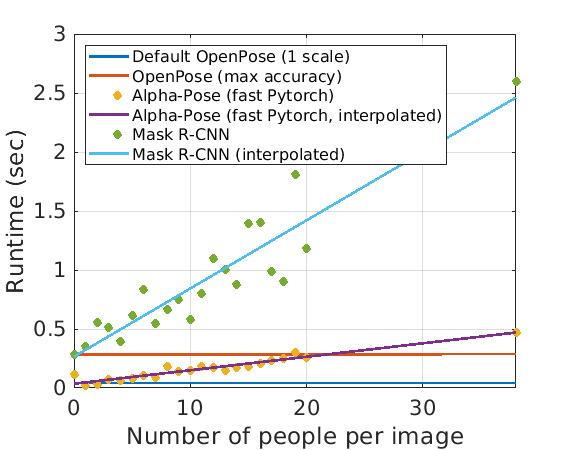
\includegraphics[width=0.6\textwidth]{Images/openpose_vs_competition.png}
    \caption{OpenPose run time for multiple\\ models and numbers of people}
    \label{fig:openpose run time}
\end{figure}

\subsection{System Pipeline}

As a recap of the processes used a step by step process of the system is
written below:\\

The complete template matching/GPU pipeline combines multiple processing steps:
\begin{enumerate}
    \item \textbf{Template preprocessing:} Load face template and compute mean-subtracted version
    \item \textbf{Frame processing:} For each input frame, compute NCC at all positions
    \item \textbf{Maximum detection:} Find location of maximum correlation (face center)
    \item \textbf{Centering calculation:} Compute translation offset to center face at frame position (width/2, height/5)
    \item \textbf{Image transformation:} Apply translation to center the user's face
\end{enumerate}

The pose estimation/CPU pipeline is below:

\begin{enumerate}
    \item \textbf{Blob creation:} The input frame is preprocessed into a blob with fixed dimensions (800x800) and normalized using mean subtraction with values [104, 117, 123]
    \item \textbf{Forward pass:} The blob is fed through the neural network
    \item \textbf{Confidence filtering:} Detections with confidence scores above 0.7 are retained
    \item \textbf{Coordinate scaling:} Bounding box coordinates are scaled back to original image dimensions
    \item \textbf{ROI is created:} Based on the bouding box a ROI is created.
    \item \textbf{ROI is downscaled:} ROI is downscaled to 368x368.
    \item \textbf{OpenPose is ran:} The output points of open pose are stored for use in the game.
\end{enumerate}

With the complete porcessing logic for pose estimation and centering of the
player the following section focuses on the game development and
implementation.

\section{Game Logic and Interaction}~\label{sec:Game Logic and Interaction}

\subsection{Game and States}

The game operates in multiple states managed through the main loop. Although
the game is always trying to be in one of these states, if the face detector
doesn't detect any faces, the game will be on stasis until a face is detected.
However, any timers that have already been started will not pause during this
stasis state.

\begin{figure}[H]
    \centering
    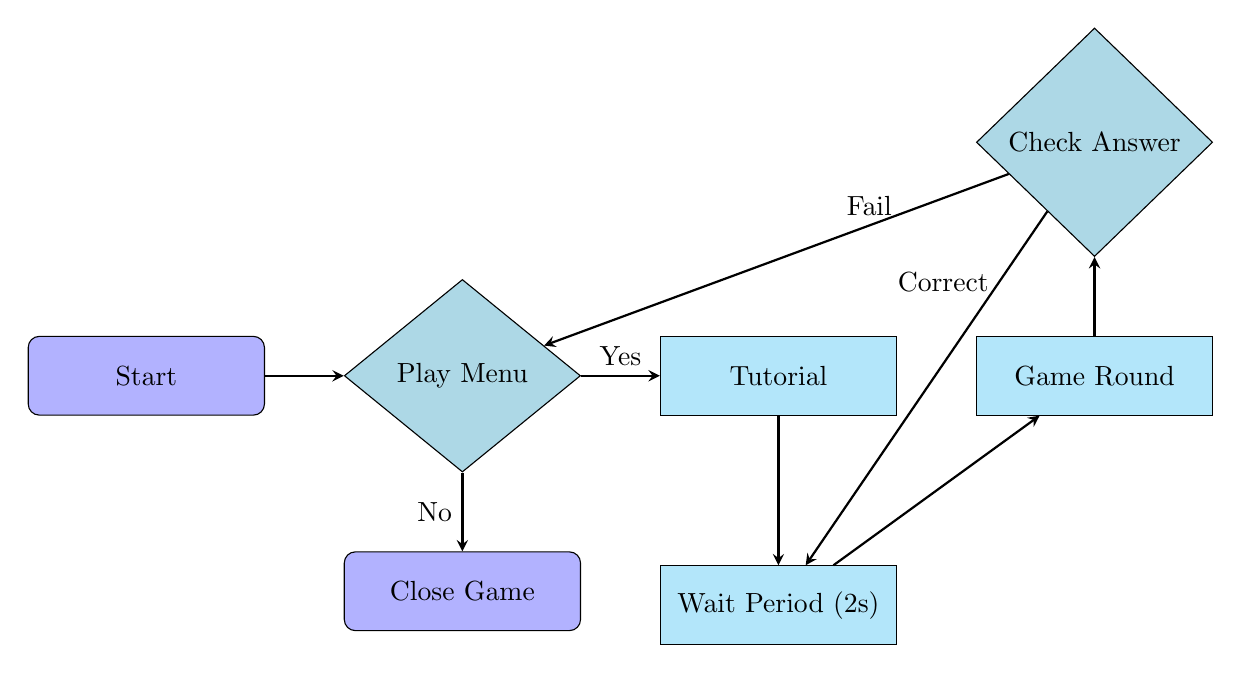
\begin{tikzpicture}[node distance=1cm]
        \node (start) [startstop] {Start};
        \node (menu) [decision, right=of start] {Play Menu};
        \node (tutorial) [process, right=of menu] {Tutorial};
        \node (game) [process, right=of tutorial] {Game Round};
        \node (wait) [process, below=1.9cm of tutorial] {Wait Period (2s)};
        \node (score) [decision, above=of game] {Check Answer};
        \node (end) [startstop, below=of menu] {Close Game};

        \draw [arrow] (start) -- (menu);
        \draw [arrow] (menu) -- node[anchor=south] {Yes} (tutorial);
        \draw [arrow] (menu) -- node[anchor=east] {No} (end);
        \draw [arrow] (tutorial) -- (wait);
        \draw [arrow] (wait) -- (game);
        \draw [arrow] (game) -- (score);
        \draw [arrow] (score) -- node[anchor=east, pos=0.2] {Correct} (wait);
        \draw [arrow] (score) -- node[anchor=south, pos = 0.3] {Fail} (menu);
    \end{tikzpicture}
    \caption{Game state machine}
    \label{fig:game_states}
\end{figure}

Before starting the game, the GameManager, the class that controlls most things
in the game loads into memory the settings that are stored in the settings.json
file. From now on when a [json] in the text it means the mentioned feature can
be adjusted inside the settings.json file, not all features that can be
adjusted through the settings.json file will be mentioned.

\subsubsection{Menu}

Whilst in the main menu state, the players are presented with a choice, either
to play the game or not. Players hover their hand over the displayed boxes to
present their choice:

\begin{itemize}
    \item \textbf{Yes box} (green, left side): Starts the game
    \item \textbf{No box} (red, right side): Exits the application
\end{itemize}

It is important to note that whilst in the menu, if the player chooses
multiuple boxes as the answer, the game will interpret that as a yes.

\subsubsection{Tutorial}

The tutorial displays instructions for 5 seconds [json] explaining the game
mechanics before transitioning to the first round. The user can choose whether
or not the tutorial is displayed [json].

\subsubsection{Game}

During active gameplay, the player is presented with a choice between 4 colored
boxes (Blue, Green, Red, Yellow) [json]. They are then presented with a word
that spells one of this 4 colors and is colored in the shade of one of these 4
colors, the player must choose the color the word is colored as, by moving
their hands inside the respective colored square, to gain points. If the player
chooses the wrong square they loose and have to start over, if the player
chooses more than one square, they loose and have to start over as well.

\paragraph{}
The color that the word spells and it's shade start of the same (if the word is
shaded Blue it also spells Blue) as the player accumulates more points the word
stops spelling the color of it's shade, and starts spelling one of the other 3
colors instead. At the same time the more rounds the player plays the shorter
time they have to answer. A player starts the game having 15 seconds to answer
    [json] and that time decreses at 0.9 rate [json] as rounds advance, (if the
player started with 15 seconds of time to answer in the first round, then in
the seconde round they will have $15 \times 0.9$ or 13.5 seconds to answer). If
a player runs out of time they loose and have to start over.

\subsection{Collision Detection}

The game checks a player choice by detecting if their hands are within the box
locations. For this the game needs to detect the body position, it does this by
detecting the player face, with a DNN model [json], then with that face's
location grabbing a subimage that contains the entire body of the person and
send that image to the pose estimator model [json] to estimate the body parts
locations. To improve performance the image sent to the pose estimator model is
downscaled to 368x368 size [json].

The pose estimator then returns the image coordinates the body parts in
question, and their positions are checked to determine what box the player
chose. In this case the body parts being check are the wrists and ankles, as
the used pose estimator model doesn't identify neither hands nor feet. If the
afformentioned body parts coordinates fall within the top left (x, y), and the
bottom right (x, y) coordinates, of a given box, then that box is considered
selected.

The game implements strict matching rules position matching:
\begin{itemize}
    \item Keypoint coordinates are scaled from 368x368 crop back to original body ROI
          dimensions
    \item Only valid (non-None) keypoints are considered
    \item Exactly one hand in correct box = success
    \item One hand in wrong box = failure
    \item Multiple hands detected = failure (prevents cheating)
\end{itemize}

\subsubsection{Text Color Probability Decay}

As mentioned before, at the beginning of the game, the color of the displayed
text is highly likely to match text itself, making early rounds easier for the
player. As the game progresses and the score increases, this probability
decreases, increasing the difficulty.

The probability of the text color matching the word color is defined as:

\begin{equation}
    P_{\text{match}} = \frac{10}{\log_{100}(\text{score} + 1)}
\end{equation}

At the start of each round, a random integer \( r \in [0, 100] \) is generated.
If \(r \leq P_{\text{match}}\) then the text color matches the word. Otherwise,
the text color is randomly selected from the remaining colors.

This logarithmic decay ensures:
\begin{itemize}
    \item Near-certain color-word matching at low scores
    \item Gradual reduction of matching probability as score increases
\end{itemize}

This implementation ensures a difficulty progression within the game,
preventing the player from feeling bored and incentivising them to improve at
the game.

\bibliography{references}

\appendix
\section{Computer Specification} \label{anex:Computer Specification}

\begin{table}[H]
    \centering
    \centering
    \begin{tabular}{|l|l|}
        \hline
        \multicolumn{2}{|c|}{\textbf{Filipe Cavalheiro}}   \\ \hline
        \textbf{Property}        & \textbf{Value}          \\ \hline
        Name                     & NVIDIA CUDA             \\ \hline
        Vendor                   & NVIDIA Corporation      \\ \hline
        Version                  & OpenCL 3.0 CUDA 13.1.86 \\ \hline
        Device Name              & NVIDIA GeForce RTX 2060 \\ \hline
        Max Compute Units        & 30                      \\ \hline
        Max Constant Args        & 9                       \\ \hline
        Max Work Item Dimensions & 3                       \\ \hline
        Max Work Item Sizes      & [1024, 1024, 64]        \\ \hline
        Max Work Group Size      & 1024                    \\ \hline
        Image Support            & 1                       \\ \hline
        Image2D Max Width        & 32768                   \\ \hline
        Image2D Max Height       & 32768                   \\ \hline
        Local Mem Size           & 49152                   \\ \hline
    \end{tabular}
\end{table}

\begin{table}[H]
    \centering
    \centering
    \begin{tabular}{|l|l|}
        \hline
        \multicolumn{2}{|c|}{\textbf{Diogo Novais}}                             \\ \hline
        \textbf{Property}                  & \textbf{Value}                     \\ \hline
        Name                               & NVIDIA CUDA                        \\ \hline
        Vendor                             & NVIDIA Corporation                 \\ \hline
        Version                            & OpenCL 3.0 CUDA 13.1.86            \\ \hline
        Device Name                        & NVIDIA GeForce RTX 5060 Laptop GPU \\ \hline
        Max Compute Units                  & 26                                 \\ \hline
        Max Constant Args                  & 9                                  \\ \hline
        Max Work Item Dimensions           & 3                                  \\ \hline
        Max Work Item Sizes                & [1024, 1024, 64]                   \\ \hline
        Max Work Group Size                & 1024                               \\ \hline
        Image Support                      & 1                                  \\ \hline
        Image2D Max Width                  & 32768                              \\ \hline
        Image2D Max Height                 & 32768                              \\ \hline
        Local Mem Size                     & 49152                              \\ \hline
        Preferred Work Group Size Multiple & 32                                 \\ \hline
    \end{tabular}
\end{table}

\section{Developed Kernels} \label{anex:Developed Kernels}

\begin{lstlisting}[language=Python, caption={kernel funcs.py}, label={annex:kernel funcs}]
import cv2 as cv
import numpy as np
import pyopencl as cl
import math
import matplotlib.pyplot as plt
from gameManager import GameManager

def subtract_template_avg(gm: GameManager, verbose: bool = False):
    face_template = cv.imread(gm.face_template_location)
    face_template_rgba = cv.cvtColor(face_template, cv.COLOR_BGR2RGBA)

    h, w, c = face_template_rgba.shape
    face_template_rgba = face_template_rgba.astype(np.float32)

    # Pre-calculate template averages
    split_img = cv.split(face_template_rgba)
    template_pre_calc = np.array([np.sum(x) / (w * h) for x in split_img])

    try:
        img_format = cl.ImageFormat(cl.channel_order.RGBA, cl.channel_type.FLOAT)

        # Create OpenCL images
        imageIn = cl.Image(gm.ctx, cl.mem_flags.READ_ONLY | cl.mem_flags.COPY_HOST_PTR, img_format, shape=(w, h), hostbuf=face_template_rgba)
        imageOut = cl.Image(gm.ctx, cl.mem_flags.WRITE_ONLY, img_format, shape=(w, h))

        # Set kernel arguments
        kernel = gm.kernel_subtract_val_to_img
        kernel.set_arg(0, np.int32(w))
        kernel.set_arg(1, np.int32(h))
        kernel.set_arg(2, template_pre_calc)
        kernel.set_arg(3, imageIn)
        kernel.set_arg(4, imageOut)

        # Enqueue kernel execution
        cl.enqueue_nd_range_kernel(gm.commQ, kernel, (w, h), None)
        gm.commQ.finish()

        # Allocate host array to copy result
        output = np.zeros((h, w, 4), dtype=np.float32)
        cl.enqueue_copy(gm.commQ, output, imageOut, origin=(0, 0, 0), region=(w, h, 1))
        gm.commQ.finish()

        if verbose:
            img_out = output.astype(np.uint8)
            img_out_rgb = cv.cvtColor(img_out, cv.COLOR_RGBA2BGR)
            
            plt.imshow(img_out_rgb)
            plt.axis('off')
            plt.show()

            img_out_gray = cv.cvtColor(img_out, cv.COLOR_RGBA2GRAY)
            cv.imshow("frame", img_out_gray)
            cv.waitKey(0)

        face_template_gray = cv.cvtColor(face_template, cv.COLOR_RGBA2GRAY)
        sum_square_template = np.sum(np.square(np.array(face_template_gray).flatten()))

        return output, sum_square_template

    except Exception as e:
        print("From subtract_template_avg error:", e)

def normalized_correlation_coefficient(input_image, template_minus_avg, template_sum_mean, gm: GameManager, verbose: bool = False):
    
    template_minus_avg = cv.cvtColor(template_minus_avg, cv.COLOR_RGBA2GRAY)
    input_image = cv.cvtColor(input_image, cv.COLOR_BGR2GRAY)

    #input_image = cv.resize(input_image, (640, 480))
    temp_h, temp_w = template_minus_avg.shape
    img_h, img_w = input_image.shape

    #images are gray scale
    img_format = cl.ImageFormat(cl.channel_order.R, cl.channel_type.FLOAT)
    img_format_uint8 = cl.ImageFormat(cl.channel_order.R, cl.channel_type.UNSIGNED_INT8)

    # Upload template
    imageIn_template = cl.create_image(
        gm.ctx,
        cl.mem_flags.READ_ONLY | cl.mem_flags.COPY_HOST_PTR,
        img_format,
        shape=(temp_w, temp_h),
        hostbuf=template_minus_avg
    )

    # Allocate device-side images
    imageIn = cl.Image(gm.ctx, cl.mem_flags.READ_ONLY, img_format, shape=(img_w, img_h))
    
    # Output correlation map
    output_buff_shape = [img_h - temp_h + 1 ,  img_w - temp_w + 1]
    output_buff = np.zeros([output_buff_shape[0], output_buff_shape[1]], dtype=np.uint8)
    imageOut = cl.create_image(
        gm.ctx,
        cl.mem_flags.WRITE_ONLY | cl.mem_flags.COPY_HOST_PTR,
        img_format_uint8,
        shape = (output_buff_shape[1], output_buff_shape[0]),
        hostbuf = output_buff
    )

    kernel = gm.kernel_ncc_tiled

    local_work_size = (8, 8)
    global_work_size = (
        math.ceil((output_buff_shape[1]) / local_work_size[0]) * local_work_size[0],
        math.ceil((output_buff_shape[0]) / local_work_size[1]) * local_work_size[1]
    )


    input_image = input_image.astype(np.float32) 
    # Update device memory for the current sub-image
    cl.enqueue_copy(gm.commQ, imageIn, input_image, origin=(0,0,0), region=(img_w, img_h, 1), is_blocking=True)

    # Kernel: Tiled Normal Correlation Coefficient (ncc_tiled)
    kernel.set_arg(0, np.int32(img_w))
    kernel.set_arg(1, np.int32(img_h))
    kernel.set_arg(2, np.float32(template_sum_mean))
    kernel.set_arg(3, imageIn)
    kernel.set_arg(4, imageIn_template)
    kernel.set_arg(5, imageOut)
    
    cl.enqueue_nd_range_kernel(gm.commQ, kernel, global_work_size, local_work_size)

    cl.enqueue_copy(gm.commQ, output_buff, imageOut, origin=(0,0,0), region=(output_buff_shape[1], output_buff_shape[0], 1))
    gm.commQ.finish()
    
    if verbose:
        print(output_buff)
        cv.imshow("frame", output_buff)
        cv.waitKey(0)

    return output_buff

def linear_transform_img(gm: GameManager, input_image: np.array, img_shift: np.array, verbose: bool = False):
    img_h, img_w = input_image.shape[:2]
    input_image = cv.cvtColor(input_image, cv.COLOR_BGR2RGBA)

    try:
        img_format_uint = cl.ImageFormat(cl.channel_order.RGBA, cl.channel_type.UNSIGNED_INT8)

        # Create OpenCL images
        imageIn = cl.Image(gm.ctx, cl.mem_flags.READ_ONLY | cl.mem_flags.COPY_HOST_PTR, 
                           img_format_uint, shape=(img_w, img_h), 
                           hostbuf=input_image)
        
        imageOut = cl.Image(gm.ctx, cl.mem_flags.WRITE_ONLY, img_format_uint, shape=(img_w, img_h))


        # Set kernel arguments
        kernel = gm.kernel_linear_transform_img
        kernel.set_arg(0, np.int32(img_w))
        kernel.set_arg(1, np.int32(img_h))
        kernel.set_arg(2, np.int32(img_shift[0]))
        kernel.set_arg(3, np.int32(img_shift[1]))
        kernel.set_arg(4, imageIn)
        kernel.set_arg(5, imageOut)

        # Enqueue kernel execution
        cl.enqueue_nd_range_kernel(gm.commQ, kernel, (img_w, img_h), None)
        gm.commQ.finish()

        # Allocate host array to copy result
        output = np.zeros((img_h, img_w, 4), dtype=np.uint8)
        cl.enqueue_copy(gm.commQ, output, imageOut, origin=(0, 0, 0), region=(img_w, img_h, 1))
        gm.commQ.finish()

        output = cv.cvtColor(output, cv.COLOR_RGBA2BGR)

        if verbose:
            plt.imshow(output)
            plt.axis('off')
            plt.show()
        return output

    except Exception as e:
        print("From linear_transform_img error:", e)
\end{lstlisting}

\begin{lstlisting}[style=CStyle, caption={prog.c}, label={annex:prog}]
__kernel void power2(__global int* arr)
{
    int i = get_global_id(0);
    if (i < 25){
        arr[i] = arr[i] * arr[i];
    }
}

__kernel void power_const(__global int* arr, int K, __global int* result)
{
    int i = get_global_id(0);
    if (i > 25)
        return;
    arr[i] = arr[i] * K;
    result[0] += arr[i];
}

__kernel void negative(__global uchar* image, int w, int h, int padding, __global uchar* imageOut)
{
    int x = get_global_id(0);
    int y = get_global_id(1);
    int idx = y * (w*3 + padding) + x*3 ;
    if ((x < w) && (y < h)) { // check if x and y are valid image coordinates
        imageOut[idx] = 255 - image[idx];
        imageOut[idx+1] = 255 - image[idx+1];
        imageOut[idx+2] = 255 - image[idx+2];
    }
}


__kernel void brightness_and_contrast(int w, int h, int padding, int brightness, float contrast, __read_only image2d_t imageIn, __global uchar4* imageOut)
{
    const sampler_t sampler = CLK_NORMALIZED_COORDS_FALSE |
                              CLK_ADDRESS_CLAMP |
                              CLK_FILTER_NEAREST;

    int x = get_global_id(0);
    int y = get_global_id(1);
    if (x >= w || y >= h) return;

    float4 pixel = read_imagef(imageIn, sampler, (int2)(x, y)) * 255.0f;

    pixel.x = clamp(mad(contrast, pixel.x, brightness), 0.0f, 255.0f);
    pixel.y = clamp(mad(contrast, pixel.y, brightness), 0.0f, 255.0f);
    pixel.z = clamp(mad(contrast, pixel.z, brightness), 0.0f, 255.0f);
    pixel.w = 255.0f;

    int idx = y * w + x;
    imageOut[idx] = (uchar4)(pixel.x, pixel.y, pixel.z, pixel.w);
}

__kernel void sobel(int w, int h,
                    __read_only image2d_t imageIn,
                    __global uchar4* imageOut)
{
    const sampler_t sampler = CLK_NORMALIZED_COORDS_FALSE |
                              CLK_ADDRESS_CLAMP_TO_EDGE |
                              CLK_FILTER_NEAREST;

    int x = get_global_id(0);
    int y = get_global_id(1);
    if (x >= w || y >= h) return;
    
    // Sobel kernels
    int Gx[3][3] = {{1, 0, -1},
                    {2, 0, -2},
                    {1, 0, -1}};
    int Gy[3][3] = {{-1, -2, -1},
                    { 0,  0,  0},
                    { 1,  2,  1}};

    uint4 gx = 0.0f, gy = 0.0f;

    for (int i = -1; i <= 1; ++i) {
        for (int j = -1; j <= 1; ++j) {
            uint4 p = read_imageui(imageIn, sampler, (int2)(x + j, y + i));
            gx += p * Gx[i+1][j+1];
            gy += p * Gy[i+1][j+1];
        }
    }

    float4 g = sqrt(convert_float4(gx*gx + gy*gy));
    g = clamp(g, 0.0f, 255.0f);
    uint4 g_uint = convert_uint4(g); 
    
    int idx = y * w + x;
    imageOut[idx] = (uchar4)(g_uint.x, g_uint.y, g_uint.z, 255); 
}
   

__kernel void subtract_val_to_img(
    int w,
    int h,
    float4 val_to_sub,
    __read_only image2d_t imageIn,
    __write_only image2d_t imageOut)
{
    const sampler_t sampler =
        CLK_NORMALIZED_COORDS_FALSE |
        CLK_ADDRESS_CLAMP_TO_EDGE |
        CLK_FILTER_NEAREST;

    int x = get_global_id(0);
    int y = get_global_id(1);
    if (x >= w || y >= h) return;

    float4 p = read_imagef(imageIn, sampler, (int2)(x, y));
    write_imagef(imageOut, (int2)(x, y), p - val_to_sub);
}

__kernel void img_mult_pix2pix(
    int w, int h,
    __read_only image2d_t imageIn_1,
    __read_only image2d_t imageIn_2,
    __write_only image2d_t out_put_mult
)
{
    const sampler_t sampler =
        CLK_NORMALIZED_COORDS_FALSE |
        CLK_ADDRESS_CLAMP_TO_EDGE |
        CLK_FILTER_NEAREST;

    int x = get_global_id(0);
    int y = get_global_id(1);

    if (x >= w || y >= h)
        return;

    float4 p_1 = read_imagef(imageIn_1, sampler, (int2)(x, y));
    float4 p_2 = read_imagef(imageIn_2, sampler, (int2)(x, y));

    float4 result = p_1 * p_2;

    write_imagef(out_put_mult, (int2)(x, y), result);
}

#define LOCAL_H 8
#define LOCAL_W 8
#define TEMP_H 105
#define TEMP_W 90

__kernel void ncc_tiled(
    int img_w,
    int img_h,
    float template_sum_mean,
    __read_only image2d_t inputImage,
    __read_only image2d_t templateImage_min_avg,
    __write_only image2d_t outputImage) 
{
    const sampler_t sampler =
        CLK_NORMALIZED_COORDS_FALSE |
        CLK_ADDRESS_CLAMP_TO_EDGE |
        CLK_FILTER_NEAREST;

    const int global_x = get_global_id(0);
    const int global_y = get_global_id(1);

    const int group_x = get_group_id(0) * LOCAL_W;
    const int group_y = get_group_id(1) * LOCAL_H;

    const int local_x = get_local_id(0);
    const int local_y = get_local_id(1);

    // Shared tile in local memory
    __local float tile[LOCAL_H + TEMP_H - 1][LOCAL_W + TEMP_W - 1];

    /* Load tile */
    for (int y = local_y; y < LOCAL_H + TEMP_H - 1; y += LOCAL_H) {
        for (int x = local_x; x < LOCAL_W + TEMP_W - 1; x += LOCAL_W) {
            int2 coord = (int2)(group_x + x, group_y + y);
            float4 pix = read_imagef(inputImage, sampler, coord);
            tile[y][x] = pix.x; // take only the first channel (grayscale)
        }
    }

    barrier(CLK_LOCAL_MEM_FENCE);

    /* Skip out-of-bounds work-items */
    if (global_x >= img_w - TEMP_W + 1 || global_y >= img_h - TEMP_H + 1) return;

    // Compute sub-image average
    float sub_img_avg = 0.0f;
    float sub_img_sum_square = 0.0f;
    for (int template_y = 0; template_y < TEMP_H; ++template_y) {
        for (int template_x = 0; template_x < TEMP_W; ++template_x) {
            sub_img_avg += tile[local_y + template_y][local_x + template_x];
            sub_img_sum_square += tile[local_y + template_y][local_x + template_x]*tile[local_y + template_y][local_x + template_x];
        }
    }
    sub_img_avg /= (TEMP_H * TEMP_W);

    // Compute correlation
    float correlation = 0.0f;
    for (int template_y = 0; template_y < TEMP_H; ++template_y) {
        for (int template_x = 0; template_x < TEMP_W; ++template_x) {
            float sub_pix = tile[local_y + template_y][local_x + template_x];
            float tmp_min_avg = read_imagef(templateImage_min_avg, sampler, (int2)(template_x, template_y)).x;
            correlation += (sub_pix - sub_img_avg) * tmp_min_avg;
        }
    }

    correlation = correlation/sqrt(template_sum_mean * sub_img_sum_square);
    correlation = (correlation + 1) * 127.5f;

    write_imageui(outputImage, (int2)(global_x, global_y), (uint4)((uint)correlation, 0, 0, 255));
}

__kernel void linear_transform_img(
    int img_w,
    int img_h,
    int shift_x,
    int shift_y,
    __read_only image2d_t inputImage,
    __write_only image2d_t outputImage) 
{
    const sampler_t sampler =
        CLK_NORMALIZED_COORDS_FALSE |
        CLK_ADDRESS_CLAMP_TO_EDGE |
        CLK_FILTER_NEAREST;

    const int global_x = get_global_id(0);
    const int global_y = get_global_id(1);

    if (global_x - shift_x <= 0 ||  global_y - shift_y <= 0 || global_x - shift_x >= img_w ||  global_y - shift_y >= img_h) return;

    uint4 pixel = read_imageui(inputImage, sampler, (int2)(global_x - shift_x, global_y - shift_y));    

    write_imageui(outputImage, (int2)(global_x, global_y), pixel);    
}

\end{lstlisting}

\end{document}